Because of the significant change made to the preconditioner, we will test if the number of partitions now will have any effect on the learned preconditioners. The number of partitions will be symmetric for the super- and subdiagonal and the number of partitions in the test will be \(\left\lbrace 1,2,3,4\right\rbrace\).

% Now that we have a preconditioner with changed structure we wil do the runs with change in partition count with one super and sub diagonal, to see if it now will improve the preconditioner or that the results will be similar to the previous testing of the type.
From the learning curves, figure \ref{fig: par super sub learning curves}, we see similar results as the previous test with different number of partitions in section \ref{sec: num par}. That is more partitions decrease the learning rate with marginal differences in outcome. With one partition count is better in one measure but worse in another. For example with 1 partition has the highest number of individual systems that has a lower solver iteration count compared to Jacobi preconditioned systems, figure \ref{fig: par super sub BvJ}, but has a worse mean and median solver iteration count compared to the learned preconditioner with 2 partitions. 

\begin{figure}[H]
    \center
    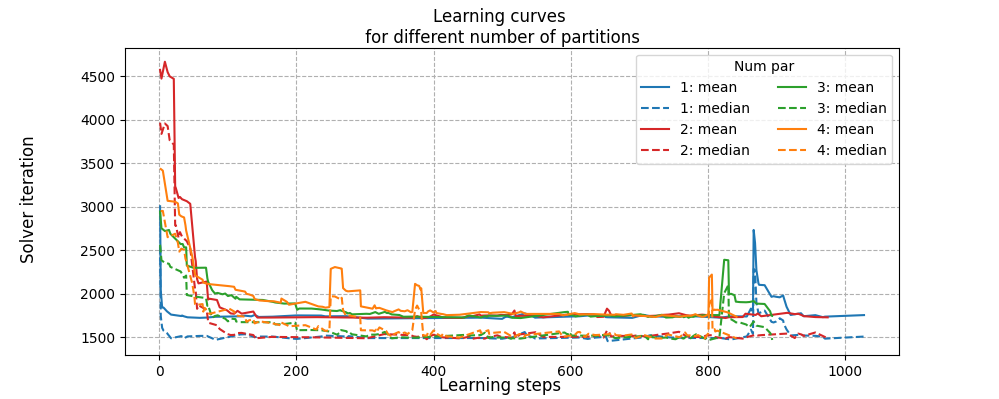
\includegraphics[width=1\textwidth]{plots/par_super_sub_learn_curve.png}
    \caption{Learning curves for learning preconditioners with 1 super- and subdiagonal. With colour corresponding to a different number of partitions and linestyle the mean or median solver iteration count.}
    \label{fig: par super sub learning curves}
\end{figure}


\begin{figure}[H]
    \center
    \begin{minipage}{.49\textwidth}
        \center
        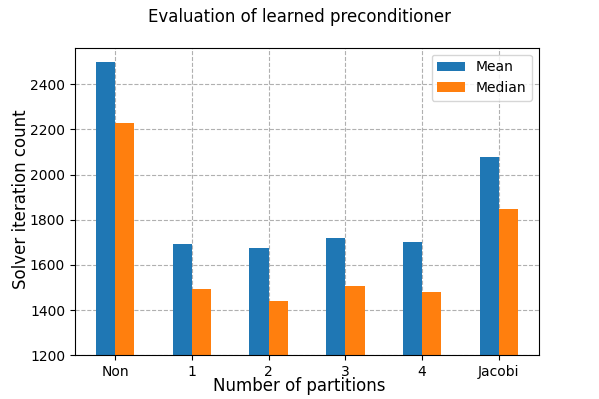
\includegraphics[width=1\textwidth]{plots/par_super_sub_test_measure.png}
        \caption{Mean (blue) and median (orange) solver iteration counts from the evaluation of the learned preconditioners, with unpreconditioned and Jacobi preconditioning for comparison.\\}
        \label{fig: par super sub test measure}
    \end{minipage}
    \begin{minipage}{.02\textwidth}
        
    \end{minipage}
    \begin{minipage}{.49\textwidth}
        \center
        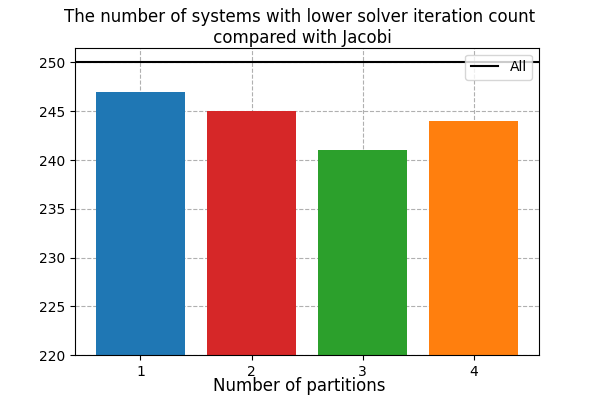
\includegraphics[width=1\textwidth]{plots/par_super_sub_BvJ.png}
        \caption{Bar Graph showing how many individual systems that has a lower solver iteration count with the learned preconditioners compared with its Jacobi preconditioned counterpart., With an y-axis offset of 220.}
        \label{fig: par super sub BvJ}
    \end{minipage}
\end{figure}


\begin{table}[H]
    \center        
    \begin{tabular}{|r|ll|}
        \hline
        Par & Superdiagonal & Subdiagonal \\ \hline
        1 & \([-0.059248]\) & \([-0.054830]\) \\
        2 & \([-0.063006, -0.064121]\) & \([-0.059046, -0.056173]\) \\ 
        3 & \([-0.064320, -0.065399, -0.058531]\) & \([-0.055929, -0.074727, -0.055672]\) \\
        4 & \([-0.046214, -0.058072, -0.047579, -0.063756]\) & \([-0.044746, -0.060495, -0.049910, -0.067014]\) \\\hline
    \end{tabular}
    \caption{Table of the learned preconditioners coefficients, with a row for each different number of partitions, columns for the superdiagonal coefficients and one for the subdiagonal coefficients.}
    \label{table: par super sub coefficients}
\end{table}

For the coefficients of the learned preconditioners, we again see similarities to section \ref{sec: num par}, that being the coefficients are similar, even between the super- and subdiagonal, table \ref{table: par super sub coefficients}. Because of this, with only slight differences in learning outcome and the faster learning we can again conclude that using 1 partition each diagonal gets better learned preconditioners.